%%%%%%%%%%%%%%%%%%%%%%%%%%%%%% -*- Mode: Latex -*- %%%%%%%%%%%%%%%%%%%%%%%%%%%%
%% 12-17.tex --  Tech report on RAs
%% Author          : Philip Johnson
%% Created On      : Mon Sep 23 11:52:28 2002
%% Last Modified By: Philip Johnson
%% Last Modified On: Mon Jun 14 12:41:23 2010
%%%%%%%%%%%%%%%%%%%%%%%%%%%%%%%%%%%%%%%%%%%%%%%%%%%%%%%%%%%%%%%%%%%%%%%%%%%%%%%
%%   Copyright (C) 2009 Philip Johnson
%%%%%%%%%%%%%%%%%%%%%%%%%%%%%%%%%%%%%%%%%%%%%%%%%%%%%%%%%%%%%%%%%%%%%%%%%%%%%%%
%% 

\documentclass[]{article}
\usepackage{graphicx}
\usepackage{cite}
\usepackage{url}
\usepackage{enumitem}
\usepackage{times}
\usepackage[margin=1in]{geometry}

% uncomment the % away on next line to produce the final camera-ready version
% and uncomment the \thispagestyle{empty} following \maketitle
%\pagestyle{empty}
\begin{document}

%\onecolumn
%\setlength{\parindent}{0cm}


\title{{\bf Looking under the lamppost for useful software analytics}} 

\author{Philip M. Johnson\\
        Collaborative Software Development Laboratory\\
        Department of Information and Computer Sciences\\
        University of Hawai`i at M\=anoa\\
        Honolulu, HI 96822\\
        johnson@hawaii.edu\\
}


\maketitle

\begin{abstract}  % 150 words
Abstract goes here.
\end{abstract}

\thispagestyle{empty}


\setlength{\parskip}{3pt plus 1pt minus 1pt} 

\section{Introduction}
Noam Chomsky once said, {\em ``Science is a bit like the joke about the drunk who is looking
under a lamppost for a key that he has lost on the other side of the street, because
that's where the light is. It has no other choice.'' \cite{Barsky98}}  For over 15 years, researchers at the
Collaborative Software Development Laboratory at the University of Hawaii have looked
for software analytics to understand and improve the process of software development, and
we believe Chomsky's scientific lamppost provides a useful metaphor for understanding
both our efforts and those of many other researchers. 

When it comes to software analytics regarding software development, in our experience
``looking under the lamppost'' is equivalent to ``collecting and analyzing metrics that
are easy to obtain with little social, political, or developmental impact.''  In other
words, the easier and less controversial a software analytic for software development, the
more constrained its usefulness and generality.  For example, the data contained in a
configuration management repository is easy to collect and the intrinsically public nature
of the repository means that few developers will object to such collection and analysis,
but such analytics inevitably provide a limited perspective on development.  On the other
hand, the original version of the Personal Software Process yields extremely rich and
impactful analytics, but entails significant overhead on developers and the analytics
themselves have significant social and political implications.

The remainder of this article discusses our work from 1995 to the present on software
analytics for software development, including research on the Personal Software Process,
Project LEAP, and three projects developed using the Hackystat Framework: Software Project
Telemetry, Zorro, and the Software Intensive Care Unit.  When put together with current
trends in the field, an interesting portrait emerges of the various trade-offs that can be
made between light and insight when looking for useful analytics about
software development.

\section{It is better to light a candle: The Personal Software Process}

Our research on software analytics for software development began in 1996 when we began
using and evaluating the Personal Software Process (PSP) as described in Watts Humphrey's
``A Discipline for Software Engineering'' \cite{Humphrey95}. This book was innovative in
several dimensions: it showed how organizational software process analytics could be
adapted to individual developers, it showed how these analytics could be used to drive
improvement, and it presented the practices in an incremental fashion amenable to
academic and professional adoption. 

\begin{figure}[!tb]
\centering
\includegraphics[width=0.95\columnwidth]{defects.eps}
\caption{Sample Defect Recording Log. In the PSP, even compiler (syntax) errors are recorded.}
\label{fig:defect-log}
\end{figure}
 
This version of the PSP uses simple spreadsheets, manual data collection, and manual
analysis. The effort required to collect and manage this data is substantial: in one
version of the PSP, developers must fill out 12 separate forms, including a project plan
summary, a time recording log, a defect recording log, a process improvement proposal, a
size estimation template, a time estimation template, a design checklist, and a code
checklist. These forms typically yield over 500 distinct values that must be manually
calculated by the developer.  Interestingly, Humphrey actively embraced the manual nature
of the PSP, writing on page 217 that ``It would be nice to have a tool to automatically
gather the PSP data. Because judgement is involved in most personal process data, no such
tool exists or is likely in the near future''.  More fundamentally, however, is the fact
that Humphrey viewed his PSP processes as simply a bootstrapping method: in Chapter 13,
``Defining the Software Process'', he exhorts developers to modify the forms and
procedures presented earlier in order to address their specific circumstances and
needs. Tool support could ``lock in'' the exemplar PSP processes, making such evolution
more difficult.

After several years of experience using the PSP, we began to worry that the manual nature
of the PSP created the potential for significant data quality problems, and performed an
empirical study that explored this issue by checking over 30,000 data values from a
classroom use of the PSP \cite{csdl-98-11}. We found that the manual nature of the PSP could
sometimes lead to incorrect process conclusions even though the overall error rate was
very low---less than 5\%. 

In retrospect, we view this original version of the PSP as ``lighting a candle'' rather
than ``looking under the lamppost'' because the approach is specifically designed to
develop custom, situationally-specific analytics. Users of the PSP may start out under the
lamppost (i.e. using the predefined PSP processes), but the approach also lights the
candle of a relatively simple, manual approach that developers can use to look for
analytics of higher value.

More specifically, the explicitly manual nature of the PSP is one of its greatest strengths,
because it empowers developers to modify and individualize the process more easily than
any of the ``advanced'' technologies to be presented below. As a simple example, consider
a developer who suspects that the number of interruptions s/he experiences each morning
directly impacts on their productivity.  The PSP provides both explicit encouragement to
explore such analytics and the lowest cost means to do so. 

\section{Project LEAP: Codifying the PSP processes} 







\section{Acknowledgements}

Acknowledge the various NSF grants. 

\bibliographystyle{plain}
\bibliography{csdl-trs,psp,hackystat,12-11}
\end{document}
